\chapter{Background}
\label{chapter:background} 

\section{JVM} %1p
\section{Software quality assurance} %2p
    The standard definition of quality assurance states it to be:
        \textit{"A planned and systematic pattern
        of all actions necessary to provide adequate confidence
        that the item or product conforms to established
        technical requirements"}~\cite{buckley1978standard}.
    Although modern \textbf{software quality assurance (SQA)} differs from the original standard definition, it is still definitely found
    at the core of SQA. To fully understand SQA and why it is important, first the software quality concept in itself is illustrated.
    Motivation for practicing SQA is examined second and third the overall activities in SQA are explained briefly.
    \subsection{Definitions of quality}
    Quality in software development is a multifaceted entity that has had many viewpoints for a long time.
    Some of these earlier views include \textit{product, transcendental, user, manufacturing} and \textit{value based} view~\cite{kitchenham1996elusive}.
    Because there exists so many viewpoints to what software quality is, it makes the measuring of quality hard~\cite{kitchenham1996elusive}.
    Business goals and their priorities should determine the needed level of software quality~\cite{kitchenham1996elusive} so therefore
    quality in itself is not set in stone, but it can alter between software services and products to fit the purpose.
    This can be easily demonstrated with an example of software inside a missile defence system or an online dating application.
    Two different systems with different goals and consequences of use and therefore obviously different standards for needed quality.

    \begin{figure}[ht]
      \begin{center}
        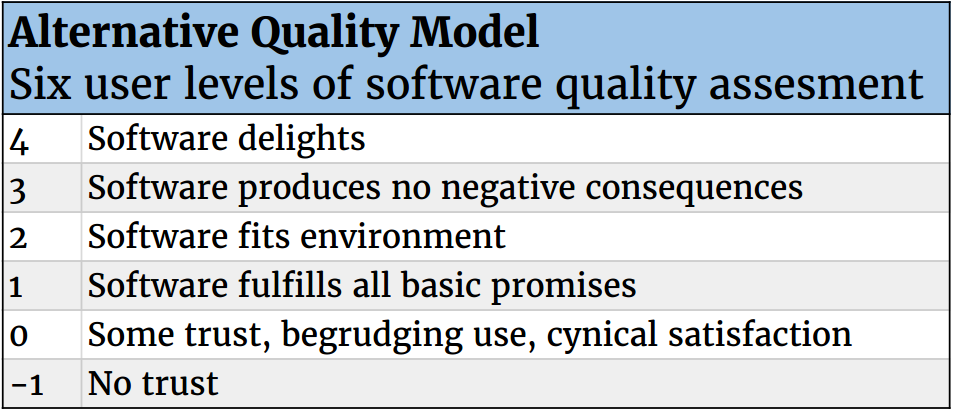
\includegraphics[width=10cm]{images/alternativeQM.png}
        \caption{Alternative Quality Model}
        \label{fig:AQM}
      \end{center}
    \end{figure}

    New alternative view on software quality by Denning~\cite{denning2016sq} includes user experience directly in the core of quality.
    This view is called the \textbf{alternative quality model (AQM)} and it defines quality software as software that delights
    the end user~\cite{denning2016sq}. Figure \ref{fig:AQM} displays the full scale of AQM.
    In my opinion, this view on software quality has strong correlation to customer value. Customer value can be seen as
    the benefits and sacrifices the end user experiences using the product~\cite{woodruff1997customer}. Therefore traditional
    defect free software quality is an important part of providing end user with software that delights, as defects
    can be seen as sacrifices that devour the trust towards software. Nevertheless this is not the only part of AQM,
    but providing software that delights the end user needs to also solve the right problem for the user.
    Thus software quality on the AQM is almost directly linked to customer value; it needs to be defect free but also
    provide benefits in use to delight the end user. While this research is mainly interested in aspects of producing traditional defect free quality software,
    later on in this chapter \textbf{Behavior Driven Development (BDD)} is examined in detail.
    BDD can be seen to directly try to increase software quality on the AQM.

    \subsection{Motivation for SQA}
    Many software projects fail but also many of them are successful. Success and failure in this context have multidimensional meaning with
    \textit{technical, economic, behavioral, psychological} and \textit{political} aspects ~\cite{mcleod2011factors}. Aggressive
    schedule can be usually seen as one of the primary causes for software project failure~\cite{cerpa2009did}. This can cause
    problems on many of the projects multidimensional axis, for instance in technical- and economical aspects. Projects might go
    over the budget, schedule, not meet the user needs and eventually be released with low quality ~\cite{cerpa2009did}.
    Although many of the problems are related to requirements engineering \textbf{(RE)}, a lot of them are fixes or rework needed after launch~\cite{lessons}.
    If quality is measured on the AQM, then both RE and SQA are intertwined in the concept of software quality and SQA-work
    is essential for the success of software project. Even if software quality is only limited to mean defect free software, SQA has
    major role in preventing project failures.

    \subsection{Activities in SQA}
    Quality assurance practices and activities differ greatly in rhythm and also to a lesser degree in practices used in
    traditional waterfall-model software projects vs agile projects~\cite{huo2004software}. Waterfall-projects have a rule set
    of their own for quality assurance, but for the topic of thesis agile methodologies and their SQA-practices are more relevant.
    SQA-practices can be generally categorized to \textit{defect detection, code enhancement, verification \& validation (V\&V)} of artifacts,
    and \textit{collaboration \& communication} between stakeholders.

    Defect detection can be split into two categories: \textbf{explicit} and \textbf{implicit} defect detection activities~\cite{mantyla2014software}.
    Implicit defect detection means finding defects as a secondary result when the goal was to perform another activity,
    such as demo presentation or giving training about the software use~\cite{mantyla2014software}. Explicit defect detection activities
    hold ones such as \textit{testing} and artifact \textit{inspection}, but they are found to have a lower
    defect detection rate than implicit ones~\cite{mantyla2014software}. \textit{Continuous integration} can also be seen
    as a explicit defect detection as it illustrates integration defects and problems with frequent integration cycle~\cite{huo2004software}.

    Code enhancement activities aim to produce better design and maintainability of the codebase and these include practices
    like \textit{pair programming, refactoring}~\cite{huo2004software} and \textit{code reviews}~\cite{rigby2013convergent}.
    Although code reviews are also a form of inspection and explicit defect detection, one of their primary uses in modern
    code review is to share knowledge between team members~\cite{mantyla2014software}~\cite{rigby2013convergent}.

    Verification \& Validation aims to guarantee the quality of product or intermediate products and it can be used for
    example to design and requirement artifacts. It is a static method, which involves stakeholder(s)
    inspecting the artifact. It is more of a traditional waterfall software project activity, but agile practices such as code reviews
    can be categorized as a V\&V activity. ~\cite{huo2004software}

    Collaboration and communication between stakeholders are used in agile methodologies frequently being one of the
    cornerstones of agile practices in general~\cite{huo2004software}. Frequent customer collaboration with \textit{On-site customer}~\cite{huo2004software}
    is an agile SQA-practice that establishes a foundation for many agile practices and is essential in delivering
    quality on the AQM.

    There are many more specific SQA-practicies that have their foundations on the activities mentioned in this section.
    Next in this thesis testing is examined in detail through automated testing as it provides a base for \textbf{Test Driven Development (TDD)}
    and BDD.

\section{Automated testing} %3p
    Agile methodologies do not prefer or deny separate testers inside a project, but for a modern quality centered
    development separate testers might hinder the experience. Teams without separate testers have one aspect in common,
    they rely heavily on test automation as the core for quality. One of the most important properties in these kind of
    teams is the rapid and direct feedback that test automation can provide. ~\cite{prechelt2016quality}

    First in this section different levels of test automation are explored. Second lower levels of test automation are explained in more
    detail and third overall benefits and drawbacks of test automation are discussed.
    \subsection{Levels of automation}
    \subsection{Low level testing explained}
    \subsection{Benefits and drawbacks}
    %Microsoft\newline
    %-20.9percent decrease in test defects\newline
    %-Cost approximately 30percent more development time\newline
    %-Relative decrease in defects found by customer in first 2 years of use\newline
    %-Developers feel more confident in refactoring and modifying code due to precense of automated unit tests\newline
\section{xUnit testing frameworks} %2p
-JUnit\newline
-Java Spring testing with with JUnit\newline
\section{Test Driven Development} %2p
    \subsection{Definition}
    \subsection{Benefits and drawbacks}
\section{Behavior Driven Development} %2p
    \subsection{Definition}
    \subsection{BDD vs TDD}
    \subsection{Levels of specification}
    \subsection{Tools}
    \subsection{Benefits and drawbacks}
\section{Behavior Driven low level testing frameworks} % 5p
    \subsection{Spec family}
            -Rspec and Spectrum\newline
            -Rspec / BDD Helps to shift viewpoint from 1-1 relationship between test-code and only one test method per function
    \subsection{Spock}
\section{Related research} % 2p
    -Analysis of problems found from automated testing surveys\newline
    -Reference to future research introduced in thesis work\newline

    Dippatyöstä TOWARDS AN EMPIRICAL EVALUATION
                OF BEHAVIOUR - DRIVEN DEVELOPMENT\newline
    -Suora lainaus: The benefits of developing a system written in a static language such as Java, while specifying its
     behaviours using a more flexible dynamic language such as JRuby could be analyzed.\newline\newline

    A Survey on Unit Testing Practices and Problems:\newline
    -Developers are striving to find realistic scenarios.\newline
    -Isolating unit under test was found hard (mocking etc)\newline
    -There clearly is potential for unit testing research to help developers produce better tests that make debugging and fixing easier\newline
    -Understanding code is bigger problem than understanding test code\newline
    --> If good tests can be generated, then these may help in understanding the code.\newline
    -Only half of the respondents enjoy writing unit tests\newline
    --> There is a need for tools that rise the enjoyment\newline
    -Maintaining unit tests is found harder than writing unit tests\newline
    --> Need for easier maintaining. Can better readability, Easy parametrization and code repetition removal practices help?\newline\newline

    Automatically Documenting Unit Test Cases:\newline
    -Majority of developers (60.38percent) found understanding of unit test cases to be at least moderately difficult\newline
    -Developers find up-to-date documentation and comments within test cases to be useful\newline
    -Writing comments to unit tests is a practice rarely or never done\newline
    -In order to effectively maintain test cases, it is important that developers understand the impact of each unit
     test case and the particular functionality that it aims to test.\newline
    -Developers feel that tests should be self-documentating\newline
    -More than half of the developers indicated a difficulty of moderate to very hard in terms of understanding unit tests.\newline
    -Emphasizing this importance, we observed that 89.15percent of developers agree or strongly agree that maintaining test cases
      impacts the quality of the system. This suggests that developers could benefit from tools that support them in maintaining unit test
       cases during software evolution and maintenance\newline\newline

   Per Runeson: A Survey of Unit Testing Practices\newline
   -Unit tests are documented in test code rather than in text\newline
   -Unit test motivation in agile: test suites could function as a specification\newline
   -Maintaining was found to take much effort\newline
   -Developer motivation working with unit tests needs improvement\newline
\section{Research hypothesis} %1p
    Discussion about research hypothesis (BD-testing vs JUnit) and how it relates to problems found (8) and benefits mentioned in section 6-7.\newline
    -Developers will write more granular test cases\newline
        %-Ubiquitous language
        %-BDD Helps to shift viewpoint from 1-1 relationship between test-code and only one test method per function
    -Developers will find easier to understand test cases\newline
        %-More comments, longer descriptions naturally in use through ubiquitous language
        %-Test Code should describe the behaviors of the object
    -Developers will find it easier to maintain code\newline
         %-Test Code should be part of system’s documentation
         %-Test Code should have less repetition
    -Developers will perceive working with low level automated testing more enjoyable\newline
